% ||||||||||||||||||||||||||||||||||||||||||||||
% Capitulo de Metodologia
% ||||||||||||||||||||||||||||||||||||||||||||||

\chapter{Metodologia}


%++++++++++++++++++++++++++++++++++++++++++++++++++++++++++++++++
% 
%++++++++++++++++++++++++++++++++++++++++++++++++++++++++++++++++

\section{Planta de Ensaio de Falhas}



%----------------------------------------------------------------
%
%----------------------------------------------------------------

\subsection{Elementos Mecânicos e Especificações}


Falar sobre: 
\begin{itemize}
    \item parâmetros da planta
    \item diferentes configurações da montagem e os ângulos para o desalinhamento
\end{itemize}

\begin{figure}[H]
    \caption{Estrutura do simulador MFS ®.}
    \begin{center}
        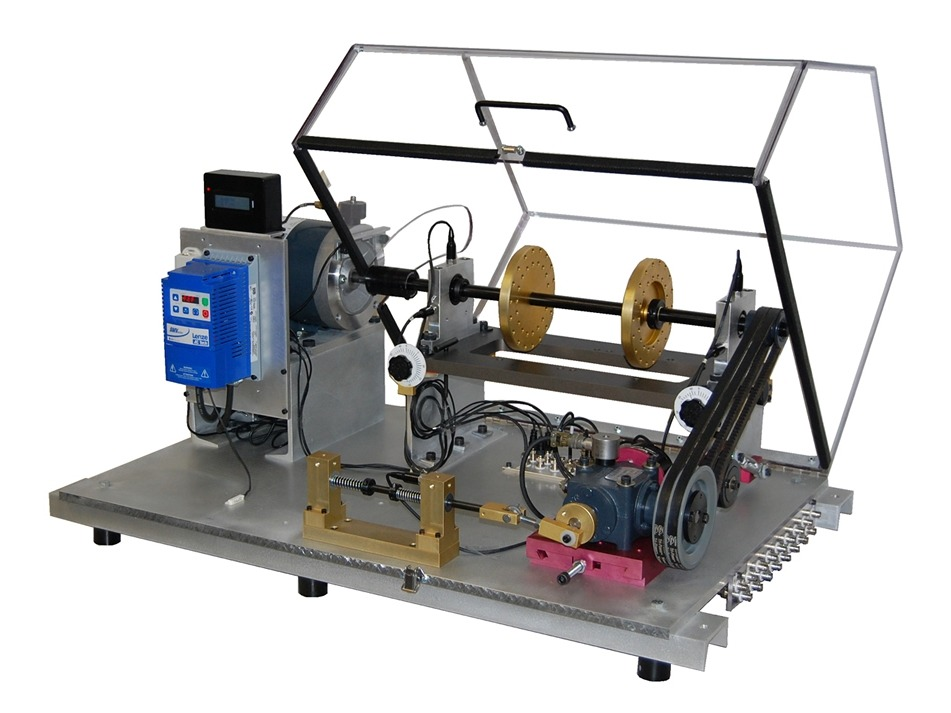
\includegraphics[scale=.4]{metodologia/img/real_plant}
    \end{center}
    \fonte{SpectraQuest ® (s.d.).} 
    \label{fig:satelite_completo}
\end{figure}


%----------------------------------------------------------------
% 
%----------------------------------------------------------------

\subsection{Aquisição dos Dados}

Falar sobre: 
\begin{itemize}
    \item Especificações dos sensores e do software VibraQuest PRO
    \item configurações do software
    \item diferentes configurações da montagem
    \item variações na frequência de amostragem e do inversor
    \item indicar as posições ods sensores na imagem abaixo 
\end{itemize}

\begin{figure}[H]
    \caption{Desenho simplificado da Planta.}
    \begin{center}
        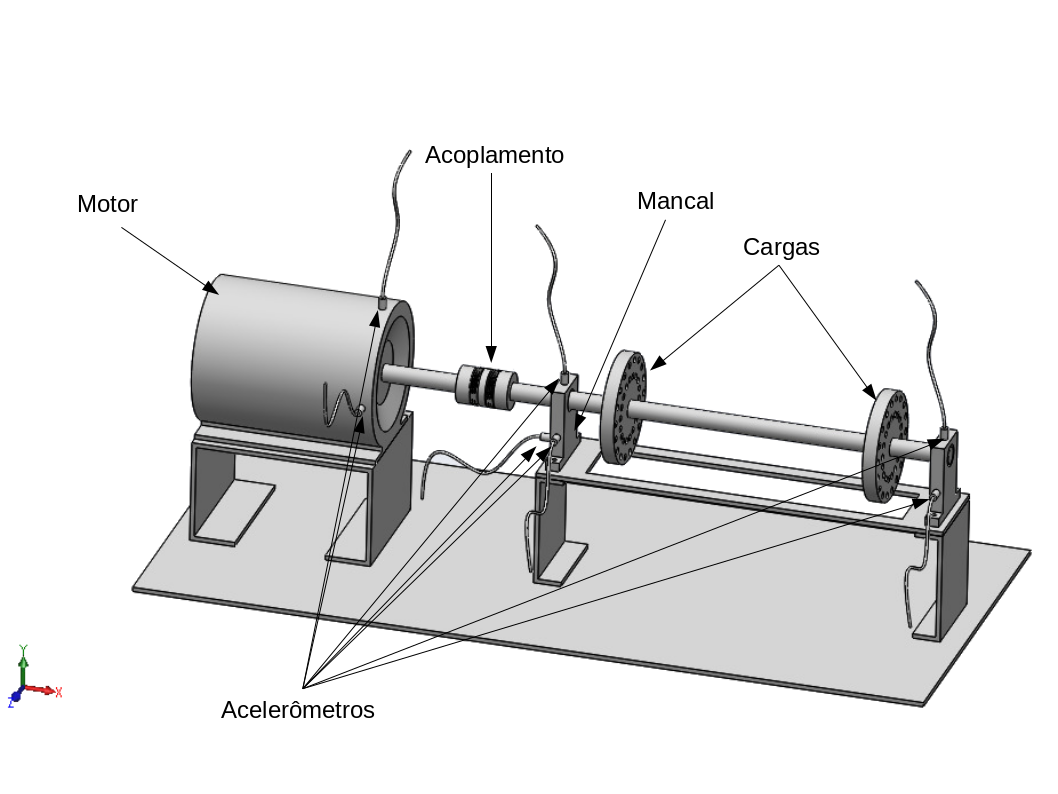
\includegraphics[scale=.5]{metodologia/img/lateral_desenho.png}
    \end{center}
    \fonte{Elaborado pelo Autor.} 
    \label{fig:}
\end{figure}
%++++++++++++++++++++++++++++++++++++++++++++++++++++++++++++++++
% 
%++++++++++++++++++++++++++++++++++++++++++++++++++++++++++++++++

\section{Processamento dos Sinais}

{breve introdução}

%----------------------------------------------------------------
%  
%----------------------------------------------------------------

\subsection{ICA}

Falar sobre: 
\begin{itemize}
    \item falar de Python
    \item fluxograma e um pouco de conceitos do porque usar
\end{itemize}

\begin{figure}[H]
    \caption{Fluxograma da técnica qe utiliza ICA.}
    \begin{center}
        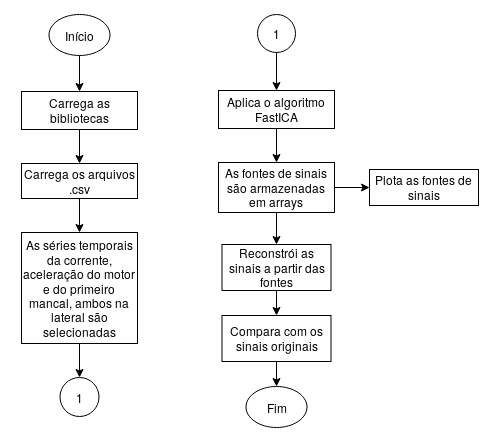
\includegraphics[scale=.65]{metodologia/img/ica.png}
    \end{center}
    \fonte{Elaborado pelo autor.} 
    \label{fig:}
\end{figure}

%----------------------------------------------------------------
%  
%----------------------------------------------------------------

\subsection{T-SNE}

Falar sobre: 
\begin{itemize}
    \item falar um pouco do conceito de clusterização neste caso
    \item fluxograma e um pouco de conceitos do porque usar
\end{itemize}

\begin{figure}[H]
    \caption{Fluxograma da técnica que utiliza t-SNE.}
    \begin{center}
        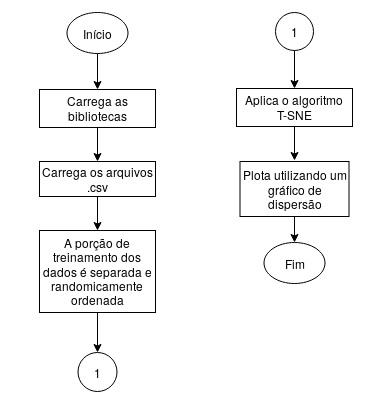
\includegraphics[scale=.65]{metodologia/img/t-sne.png}
    \end{center}
    \fonte{Elaborado pelo autor.} 
    \label{fig:}
\end{figure}

%----------------------------------------------------------------
%  
%----------------------------------------------------------------

\subsection{K-Means}

Falar sobre: 
\begin{itemize}
    \item Falar de R
    \item falar um pouco do conceito de clusterização neste caso
    \item fluxograma e um pouco de conceitos do porque usar
\end{itemize}

\begin{figure}[H]
    \caption{Fluxograma da técnica utilizando K-means.}
    \begin{center}
        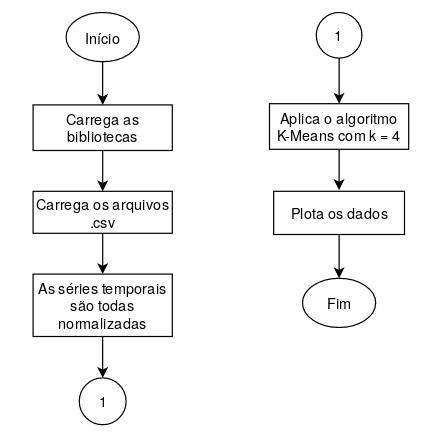
\includegraphics[scale=.65]{metodologia/img/k-means.png}
    \end{center}
    \fonte{Elaborado pelo autor.} 
    \label{fig:}
\end{figure}